\documentclass[11pt,a4paper]{article}
\usepackage[utf8]{inputenc}
\usepackage[T1]{fontenc}
\usepackage{amsmath}
\usepackage{amssymb}
\usepackage{graphicx}
\usepackage{booktabs}
\usepackage{hyperref}
\usepackage{geometry}
\geometry{margin=0.8in}

\title{Understanding Context Sampling in TabPFN\\ on Small Tabular Datasets}

\author{
  Mohammed Abdullah\\
  Department of AI \& Data Science\\
  Anna University\\
  \texttt{2023176026@student.annauniv.edu}
}

\date{\today}

\begin{document}

\maketitle

\begin{abstract}
TabPFN classifies by in-context learning: it conditions on a set of labeled
training rows (the context, or prototypes) and predicts test labels without
gradient updates. On small tabular datasets, where TabPFN is designed to be
used, the practitioner still chooses how large that context is and which rows
go into it. We ask how much those choices matter. Using repeated random
sub-sampling on 15 small OpenML datasets, we study three linked questions:
(i) how variable predictions are across different random contexts of the same
size, and whether larger contexts are more stable; (ii) whether accuracy tracks
how well a sampled context preserves the full training distribution; and
(iii) whether more expensive selection (K-Means, farthest-point sampling) buys
anything over uniform random selection once the context is representative.
We find that larger contexts are both more accurate and markedly more stable
(the coefficient of variation of AUC falls from roughly 6--18\% at $k{=}16$ to
1--4\% at the largest $k$ on the datasets with room to improve). Accuracy does
correlate with how well a random context preserves the training distribution,
but a controlled experiment overturns the causal reading: when we construct
contexts that match the feature means closely, accuracy drops substantially (by
up to 0.5 AUC), because that construction also destroys diversity. Controlled
experiments and mixed-effects analysis identify diversity/coverage---not
feature-mean matching---as the factor that predicts accuracy (diversity
$\beta=+0.23$, $p=3\times10^{-12}$; feature-mean shift $\beta=-0.01$, $p=0.71$
once diversity is included). This also explains why K-Means and farthest-point
selection---diverse but not distribution-preserving---match uniform random while
costing two to three orders of magnitude more. Random sampling works because it
covers the feature space in expectation, not because it matches its
distribution. We report effect sizes and confidence intervals throughout.

\textbf{Keywords:} in-context learning, TabPFN, prototype sampling, context
diversity, coverage, context stability, small data
\end{abstract}

\section{Introduction}

Prototype selection is a fundamental inference-time decision in TabPFN: the
model conditions on a chosen set of labeled rows (the context) and predicts in a
single forward pass. Sophisticated selection methods (clustering, coverage
heuristics) have been proposed, yet it remains unclear whether their gains come
from the selection \emph{algorithm} or simply from selecting a subset that is
representative of the training data. We investigate this on small tabular
datasets---the regime TabPFN targets---where we can afford many repeated draws
and isolate the effect of the context from confounds of scale.

We study three connected questions, on 15 small OpenML datasets:

\begin{description}
\item[H1 (Stability).] Different random contexts of the same size $k$ yield
different predictions; the spread of accuracy across random draws shrinks as $k$
grows.
\item[H2 (What makes a context good).] We ask whether accuracy is driven by how
well the context preserves the training distribution (representativeness) or by
how well it covers the feature space (diversity). A correlation initially
suggests representativeness; a controlled experiment shows the causal factor is
diversity.
\item[H3 (Selection cost).] Expensive selection methods (K-Means, FPS) add
little accuracy over uniform random selection despite far higher cost.
\end{description}

These are mechanistic questions about \emph{how} TabPFN responds to its context,
and together they form a single account: context size controls reliability (H1),
diversity/coverage---not distribution matching---explains which contexts succeed
(H2), and this explains why cheap random sampling, which covers the space in
expectation, is hard to beat (H3). We answer them with repeated random
sub-sampling, \emph{controlled} construction of contexts with targeted geometry,
and two supporting stress tests (duplicating and dropping part of the context).
Our contribution is to identify context diversity, rather than representativeness
or the choice of selection algorithm, as what a small-data context needs---and to
reach that conclusion by a controlled experiment that overturns the more obvious
correlational story.

\section{Setup}

We use TabPFN v3 with \texttt{ignore\_pretraining\_limits=True}. Each dataset is
split 80/20 (stratified, fixed split seed). A context of size $k$ is formed by
selecting $k$ training rows and fitting TabPFN on exactly those rows
(\texttt{clf.fit(X[idx], y[idx])}); the held-out 20\% is the test set throughout.
We report ROC AUC (one-vs-rest macro for the multiclass dataset). For the
stability and correlational analyses we draw \textbf{20 independent random
contexts} per $k$. For the causal analyses in H2 we additionally \emph{construct}
contexts with targeted geometry (Section on the controlled test) rather than
sampling them; for selection-method and stress tests we use three or more seeds.

\begin{table}[h]
\centering
\caption{Datasets (all small; public OpenML).}
\label{tab:datasets}
\begin{tabular}{lrrr}
\toprule
Dataset & rows & features & classes \\
\midrule
diabetes           & 768  & 8  & 2 \\
credit-g           & 1000 & 20 & 2 \\
vehicle            & 846  & 18 & 4 \\
wdbc               & 569  & 30 & 2 \\
breast-w           & 699  & 9  & 2 \\
blood-transfusion  & 748  & 4  & 2 \\
ionosphere         & 351  & 34 & 2 \\
sonar              & 208  & 60 & 2 \\
glass              & 214  & 9  & 6 \\
australian         & 690  & 14 & 2 \\
heart-statlog      & 270  & 13 & 2 \\
segment            & 2310 & 18 & 7 \\
waveform-5000      & 5000 & 40 & 3 \\
spambase           & 4601 & 57 & 2 \\
kc1                & 2109 & 21 & 2 \\
\bottomrule
\end{tabular}
\end{table}

\textbf{Context descriptors.} We characterize a context with two families of
measures on standardized features. \emph{Representativeness} (how close to the
full distribution): the total-variation distance between the context's and the
full class distribution (\texttt{class\_tv}), and the mean absolute difference
between the context's per-feature means and the full training means
(\texttt{feat\_shift})---smaller means more representative. \emph{Diversity /
coverage} (how much of the space the context spans): the mean pairwise Euclidean
distance among context rows, and the log-determinant of the context covariance
(a volume). These are standard geometric coverage measures---mean pairwise
distance summarizes spread, and the covariance log-determinant is the standard
volume of the region a point set occupies (it appears, for example, in
D-optimal experimental design and determinantal point processes). These two
families can vary independently, and separating them is the crux of H2.

\section{H1: Context Stability}

For each $k$ we drew 20 independent random contexts and recorded the resulting
test AUC. Table~\ref{tab:stability} reports the mean $\pm$ 95\% CI, and
Table~\ref{tab:stability_cv} the coefficient of variation
$\mathrm{CV}=\sigma/\mu$---a scale-free measure of variability---as a percentage.
Figure~\ref{fig:stability} plots mean AUC and CV against $k$.

\begin{table}[h]
\centering
\caption{Mean ROC AUC $\pm$ 95\% CI across 20 random contexts per $k$.
Dashes: $k{=}256$ exceeds the training-set size on the smallest datasets.}
\label{tab:stability}
\begin{tabular}{lrrrrr}
\toprule
Dataset & $k{=}16$ & $k{=}32$ & $k{=}64$ & $k{=}128$ & $k{=}256$ \\
\midrule
diabetes           & $.738{\pm}.042$ & $.788{\pm}.034$ & $.834{\pm}.008$ & $.858{\pm}.006$ & $.872{\pm}.005$ \\
credit-g           & $.648{\pm}.030$ & $.678{\pm}.027$ & $.734{\pm}.021$ & $.774{\pm}.013$ & $.808{\pm}.008$ \\
vehicle            & $.763{\pm}.022$ & $.870{\pm}.007$ & $.920{\pm}.008$ & $.946{\pm}.005$ & $.960{\pm}.002$ \\
wdbc               & $.955{\pm}.024$ & $.980{\pm}.004$ & $.987{\pm}.004$ & $.990{\pm}.002$ & $.995{\pm}.001$ \\
breast-w           & $.988{\pm}.003$ & $.989{\pm}.003$ & $.992{\pm}.002$ & $.993{\pm}.002$ & $.994{\pm}.001$ \\
blood-transfusion  & $.628{\pm}.033$ & $.644{\pm}.027$ & $.670{\pm}.015$ & $.690{\pm}.012$ & $.698{\pm}.011$ \\
ionosphere         & $.882{\pm}.035$ & $.957{\pm}.010$ & $.972{\pm}.004$ & $.980{\pm}.002$ & $.984{\pm}.001$ \\
sonar              & $.744{\pm}.036$ & $.776{\pm}.032$ & $.823{\pm}.016$ & $.899{\pm}.008$ & --- \\
glass              & $.824{\pm}.080$ & $.854{\pm}.018$ & $.917{\pm}.013$ & $.950{\pm}.005$ & --- \\
australian         & $.862{\pm}.029$ & $.906{\pm}.007$ & $.916{\pm}.006$ & $.923{\pm}.005$ & $.932{\pm}.004$ \\
heart-statlog      & $.824{\pm}.026$ & $.847{\pm}.018$ & $.854{\pm}.015$ & $.869{\pm}.006$ & --- \\
segment            & $.950{\pm}.010$ & $.980{\pm}.004$ & $.991{\pm}.001$ & $.994{\pm}.001$ & $.996{\pm}.001$ \\
waveform-5000      & $.829{\pm}.023$ & $.891{\pm}.019$ & $.945{\pm}.005$ & $.962{\pm}.002$ & $.969{\pm}.001$ \\
spambase           & $.913{\pm}.012$ & $.945{\pm}.008$ & $.966{\pm}.003$ & $.976{\pm}.001$ & $.981{\pm}.001$ \\
kc1                & $.709{\pm}.058$ & $.746{\pm}.029$ & $.778{\pm}.017$ & $.796{\pm}.014$ & $.816{\pm}.007$ \\
\bottomrule
\end{tabular}
\end{table}

\begin{table}[h]
\centering
\caption{Coefficient of variation ($\mathrm{CV}=\sigma/\mu$, \%) of ROC AUC
across the same 20 random contexts. CV falls as $k$ grows on every dataset.}
\label{tab:stability_cv}
\begin{tabular}{lrrrrr}
\toprule
Dataset & $k{=}16$ & $k{=}32$ & $k{=}64$ & $k{=}128$ & $k{=}256$ \\
\midrule
diabetes           & 12.9 & 9.7 & 2.1 & 1.7 & 1.3 \\
credit-g           & 10.5 & 9.0 & 6.5 & 3.8 & 2.1 \\
vehicle            & 6.5 & 1.9 & 2.1 & 1.1 & 0.5 \\
wdbc               & 5.8 & 0.8 & 0.8 & 0.6 & 0.2 \\
breast-w           & 0.6 & 0.8 & 0.4 & 0.4 & 0.2 \\
blood-transfusion  & 11.9 & 9.5 & 5.2 & 4.0 & 3.5 \\
ionosphere         & 8.9 & 2.3 & 1.0 & 0.5 & 0.3 \\
sonar              & 11.0 & 9.3 & 4.5 & 1.9 & --- \\
glass              & 8.6 & 4.6 & 3.3 & 1.3 & --- \\
australian         & 7.7 & 1.8 & 1.4 & 1.3 & 1.0 \\
heart-statlog      & 7.1 & 4.7 & 4.0 & 1.5 & --- \\
segment            & 1.5 & 1.0 & 0.2 & 0.1 & 0.1 \\
waveform-5000      & 6.2 & 4.9 & 1.3 & 0.5 & 0.3 \\
spambase           & 2.9 & 2.0 & 0.7 & 0.3 & 0.3 \\
kc1                & 17.8 & 8.9 & 5.0 & 4.0 & 1.9 \\
\bottomrule
\end{tabular}
\end{table}

\begin{figure}[h]
\centering
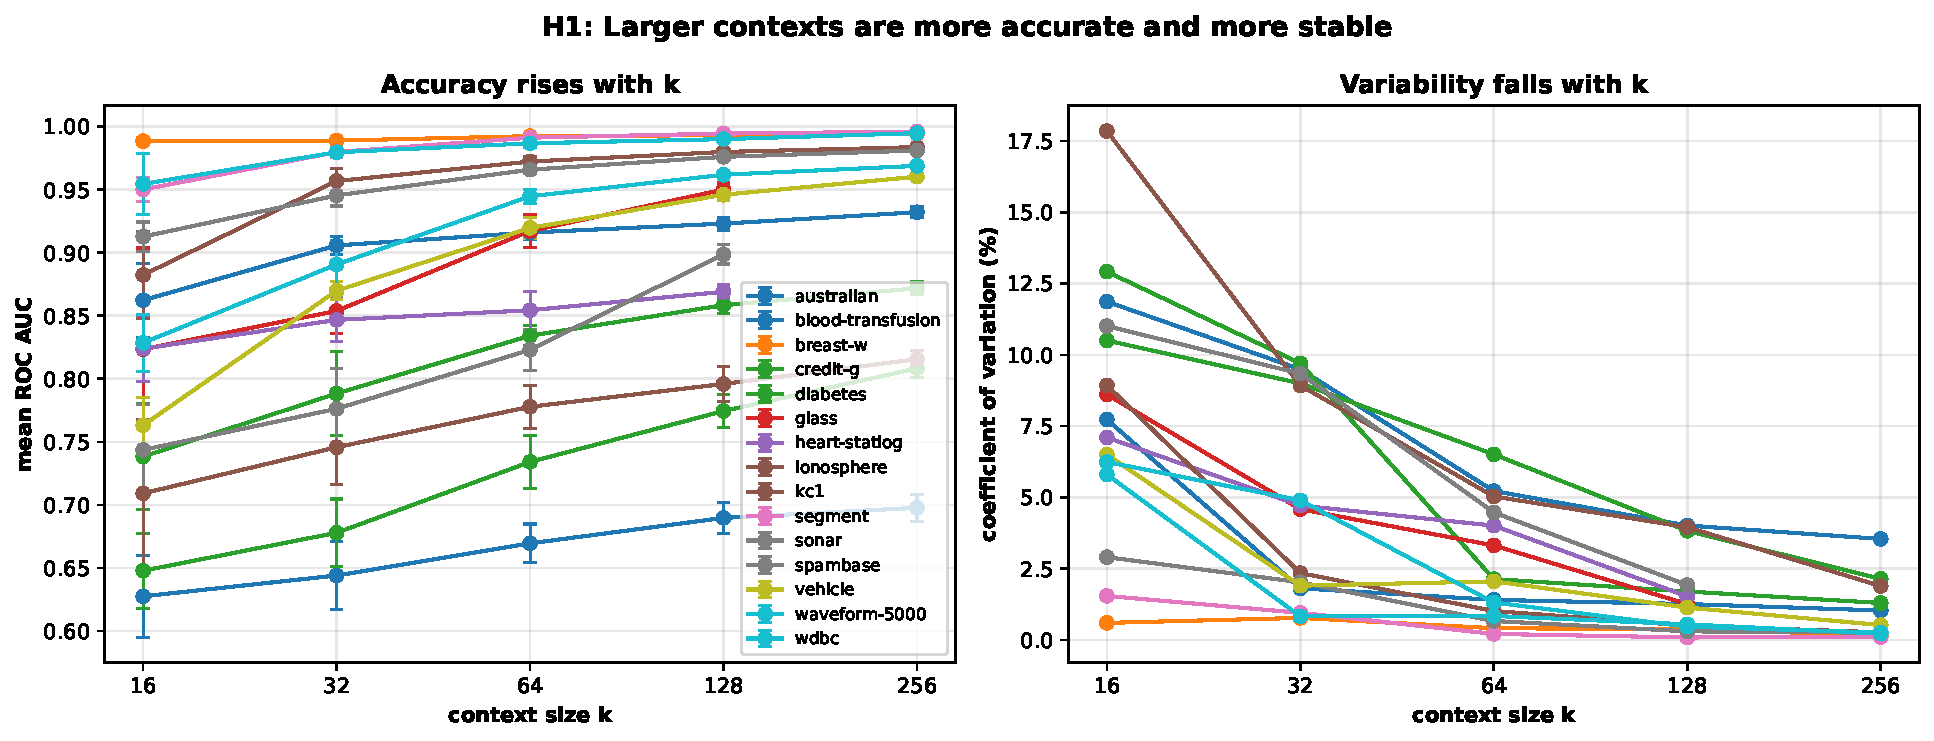
\includegraphics[width=\textwidth]{figures/p2_fig1_stability.pdf}
\caption{Mean AUC (left) rises with context size $k$; the coefficient of
variation across 20 random draws (right) falls with $k$ on every dataset.}
\label{fig:stability}
\end{figure}

\textbf{What we observe.} On every one of the 15 datasets, variability across
random contexts falls as $k$ grows. On datasets with accuracy headroom
(diabetes, credit-g, sonar, kc1, waveform, and others) the CV drops from roughly
6--18\% at $k{=}16$ to about 1--4\% at the largest $k$; datasets already near
ceiling (breast-w, segment) start low and still shrink. Mean AUC rises with $k$
in parallel. So on small data the context size is not only an accuracy knob but a
\emph{reliability} knob: a small context makes the model's answer depend heavily
on which rows happened to be drawn, and enlarging the context removes most of
that dependence. The most variable configuration we saw was kc1 at $k{=}16$
(CV $17.8\%$); at $k{=}16$ diabetes AUC over 20 draws ranged from 0.503 to 0.839.

\section{H2: What makes a context good---representativeness or diversity?}

H2 as we first posed it---that a context which preserves the full training
distribution scores higher---turns out to be the wrong reading of a real
correlation. This section builds the case in three steps: the correlation
(observed), a controlled test that overturns its causal interpretation, and a
disentangling experiment that identifies context \emph{diversity/coverage}, not
distribution matching, as the factor that actually tracks accuracy.

Using the 20 random draws per $k$ from H1, we first ask whether the draws that
better preserve the full training distribution score higher. For each draw we
computed two distances to the full training set: the total-variation distance
between class distributions (\texttt{class\_tv}) and the mean absolute
standardized feature-mean shift (\texttt{feat\_shift}). Table~\ref{tab:repr}
reports Pearson $r$, Spearman $\rho$, and linear $R^2$ per dataset, pooled over
$k$.

\begin{table}[h]
\centering
\caption{Correlation between distribution distance and AUC (all draws pooled
over $k$, per dataset). Negative values mean that a context further from the
full distribution scores lower, as hypothesized.}
\label{tab:repr}
\begin{tabular}{lrrrrrr}
\toprule
& \multicolumn{3}{c}{\texttt{class\_tv}} & \multicolumn{3}{c}{\texttt{feat\_shift}} \\
\cmidrule(lr){2-4}\cmidrule(lr){5-7}
Dataset & Pearson & Spearman & $R^2$ & Pearson & Spearman & $R^2$ \\
\midrule
diabetes           & $-0.31$ & $-0.45$ & 0.10 & $-0.52$ & $-0.73$ & 0.27 \\
credit-g           & $-0.53$ & $-0.43$ & 0.28 & $-0.80$ & $-0.83$ & 0.63 \\
vehicle            & $-0.71$ & $-0.78$ & 0.51 & $-0.79$ & $-0.78$ & 0.63 \\
wdbc               & $-0.24$ & $-0.35$ & 0.06 & $-0.39$ & $-0.59$ & 0.15 \\
breast-w           & $-0.18$ & $-0.16$ & 0.03 & $-0.18$ & $-0.27$ & 0.03 \\
blood-transfusion  & $-0.08$ & $-0.18$ & 0.01 & $-0.31$ & $-0.27$ & 0.09 \\
ionosphere         & $-0.26$ & $-0.51$ & 0.07 & $-0.63$ & $-0.84$ & 0.39 \\
sonar              & $-0.53$ & $-0.54$ & 0.28 & $-0.60$ & $-0.66$ & 0.36 \\
glass              & $-0.57$ & $-0.63$ & 0.33 & $-0.56$ & $-0.69$ & 0.32 \\
australian         & $-0.34$ & $-0.26$ & 0.11 & $-0.57$ & $-0.68$ & 0.32 \\
heart-statlog      & $-0.07$ & $-0.23$ & 0.01 & $-0.30$ & $-0.26$ & 0.09 \\
segment            & $-0.77$ & $-0.84$ & 0.59 & $-0.74$ & $-0.82$ & 0.55 \\
waveform-5000      & $-0.71$ & $-0.80$ & 0.51 & $-0.83$ & $-0.92$ & 0.68 \\
spambase           & $-0.39$ & $-0.49$ & 0.15 & $-0.78$ & $-0.89$ & 0.60 \\
kc1                & $-0.08$ & $-0.27$ & 0.01 & $-0.29$ & $-0.38$ & 0.08 \\
\midrule
pooled (z-scored)  & $-0.38$ & $-0.46$ & 0.14 & $-0.55$ & $-0.64$ & 0.31 \\
\bottomrule
\end{tabular}
\end{table}

\begin{table}[h]
\centering
\caption{Mean AUC of the most- vs.\ least-representative third of random draws,
split by \texttt{class\_tv}. The most-representative third wins on all 15
datasets.}
\label{tab:contrast}
\begin{tabular}{lrrr}
\toprule
Dataset & most repr. & least repr. & $\Delta$ \\
\midrule
vehicle           & 0.953 & 0.825 & $+0.127$ \\
sonar             & 0.858 & 0.746 & $+0.112$ \\
waveform-5000     & 0.956 & 0.867 & $+0.088$ \\
glass             & 0.942 & 0.864 & $+0.077$ \\
credit-g          & 0.752 & 0.678 & $+0.074$ \\
diabetes          & 0.851 & 0.791 & $+0.060$ \\
\multicolumn{4}{l}{\textit{\dots (remaining 9 datasets $\Delta$ from $+0.027$ down to $+0.004$)}} \\
breast-w          & 0.994 & 0.990 & $+0.004$ \\
\bottomrule
\end{tabular}
\end{table}

\begin{figure}[h]
\centering
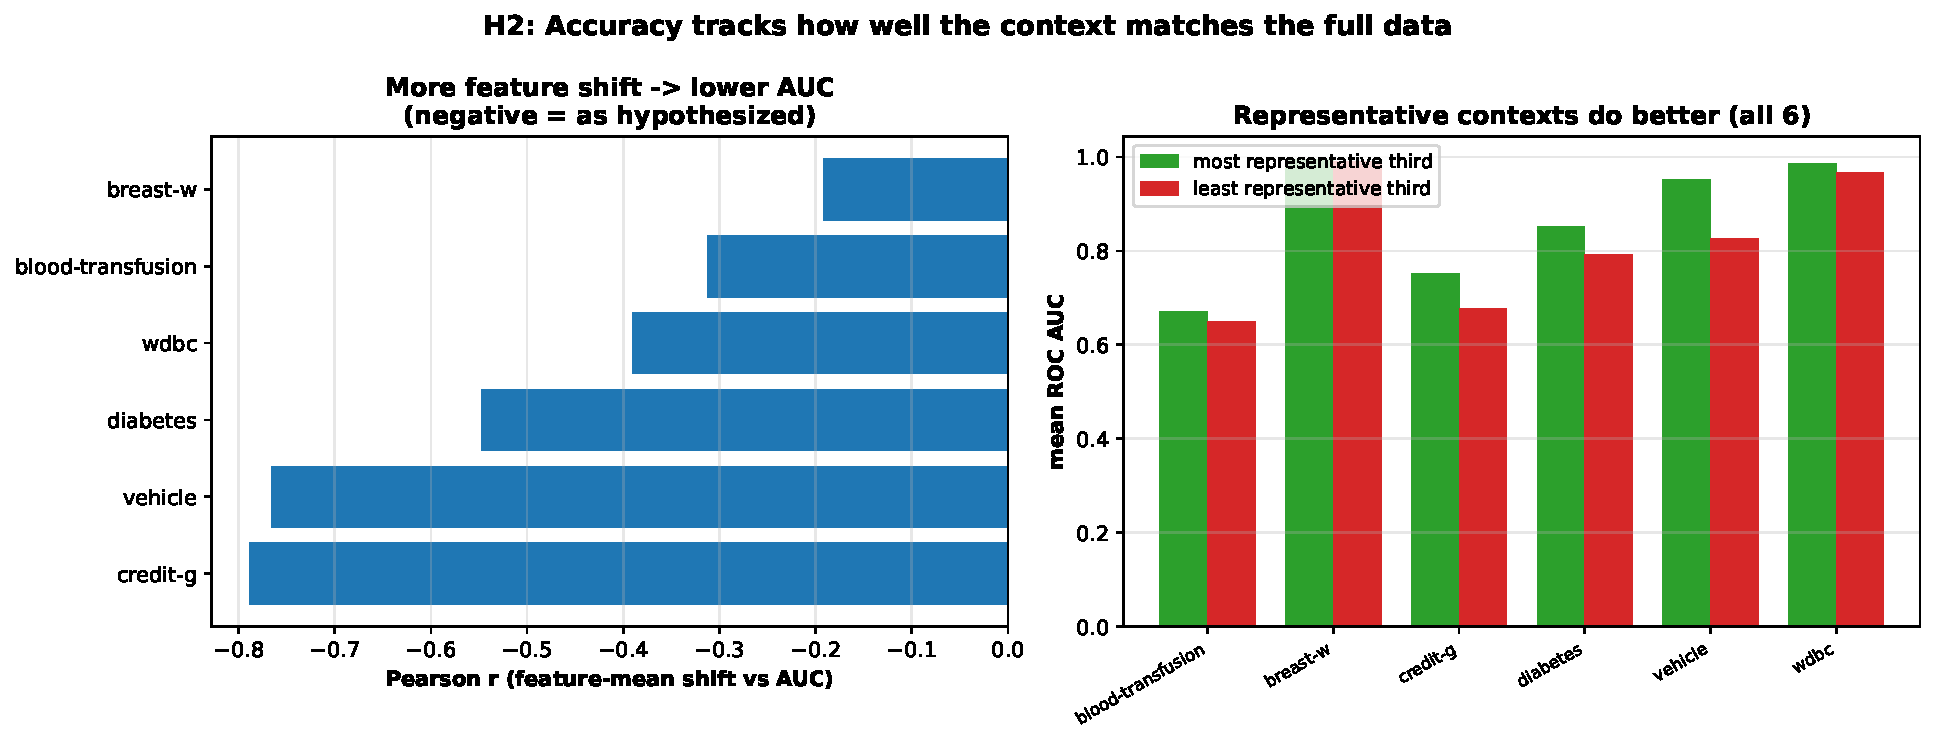
\includegraphics[width=\textwidth]{figures/p2_fig2_representativeness.pdf}
\caption{The correlational step (later overturned as causal). Left: Pearson
correlation between feature-mean shift and AUC across random draws per dataset
(all negative). Right: mean AUC of the most- vs.\ least-representative third of
random draws. This association is real but confounded with diversity, as the
controlled experiment shows.}
\label{fig:repr}
\end{figure}

\textbf{The correlation.} Across random draws, the direction predicted by H2
holds everywhere: all 15 correlations in Table~\ref{tab:repr} are negative
(further from the full distribution $\rightarrow$ lower AUC), and in
Table~\ref{tab:contrast} the most-representative third of draws beats the
least-representative third on all 15 datasets. \texttt{feat\_shift} is the
stronger predictor (pooled Pearson $-0.55$, $R^2=0.31$), and strong on several
datasets---waveform-5000 ($r=-0.83$, $R^2=0.68$), credit-g ($r=-0.80$), vehicle
($r=-0.79$), spambase ($r=-0.78$)---while weaker near ceiling (breast-w) or on
noisy datasets (kc1, heart-statlog). Taken alone, this looks like support for
H2. It is not, and the rest of this section explains why.

\subsection{A controlled test overturns the causal reading}

Correlation among random draws cannot separate cause from confound. We therefore
\emph{constructed} contexts at target representativeness levels rather than
waiting for random draws to vary: a greedy procedure that adds rows to keep the
running feature-mean as close as possible to the full-data mean (``high''
representativeness, very low \texttt{feat\_shift}), a uniform ``random''
baseline, and a farthest-from-centroid procedure (``low'' representativeness,
high \texttt{feat\_shift}), all with the class ratio matched. These constructed
contexts are designed to isolate causal factors, not to model practical sampling
strategies; their purpose is to move one geometric property at a time. If
representativeness caused accuracy, the low-shift contexts should score highest.

The opposite happens (Table~\ref{tab:controlled}). Forcing low
\texttt{feat\_shift} reduces accuracy substantially---to 0.49 on diabetes and
0.39 on blood-transfusion, far below random---while the high-shift contexts are
as good as or better than random. On most datasets the high-vs-low effect is
large and runs contrary to the original hypothesis (Cohen's $d$ up to $-22.6$,
Cliff's $\delta=-1.0$ on six datasets). So matching the marginal feature means
does not cause good performance; when isolated, it usually degrades it.

\begin{table}[h]
\centering
\caption{Controlled representativeness at $k{=}128$ (15 contexts each, mean ROC
AUC $\pm$ 95\% CI). Forcing low feature-mean shift (``high repr.'') reduces
accuracy substantially; $d$ and $\delta$ are the high-vs-low effect sizes.}
\label{tab:controlled}
\begin{tabular}{lrrrrr}
\toprule
Dataset & high repr. & random & low repr. & Cohen $d$ & Cliff $\delta$ \\
\midrule
diabetes           & $.488{\pm}.027$ & $.859{\pm}.009$ & $.861{\pm}.003$ & $-9.1$ & $-1.00$ \\
credit-g           & $.601{\pm}.024$ & $.765{\pm}.016$ & $.708{\pm}.008$ & $-3.0$ & $-0.97$ \\
vehicle            & $.910{\pm}.007$ & $.945{\pm}.004$ & $.906{\pm}.006$ & $+0.3$ & $+0.26$ \\
wdbc               & $.991{\pm}.001$ & $.992{\pm}.002$ & $.980{\pm}.001$ & $+4.8$ & $+1.00$ \\
breast-w           & $.963{\pm}.001$ & $.994{\pm}.001$ & $.992{\pm}.001$ & $-22.6$ & $-1.00$ \\
blood-transfusion  & $.389{\pm}.016$ & $.694{\pm}.009$ & $.732{\pm}.004$ & $-14.2$ & $-1.00$ \\
ionosphere         & $.966{\pm}.002$ & $.980{\pm}.003$ & $.972{\pm}.003$ & $-1.2$ & $-0.55$ \\
sonar              & $.908{\pm}.004$ & $.893{\pm}.005$ & $.897{\pm}.003$ & $+1.6$ & $+0.76$ \\
glass              & $.953{\pm}.006$ & $.950{\pm}.005$ & $.931{\pm}.002$ & $+2.4$ & $+0.99$ \\
australian         & $.777{\pm}.029$ & $.925{\pm}.007$ & $.929{\pm}.003$ & $-3.5$ & $-1.00$ \\
heart-statlog      & $.866{\pm}.003$ & $.872{\pm}.006$ & $.868{\pm}.004$ & $-0.2$ & $-0.09$ \\
segment            & $.975{\pm}.003$ & $.994{\pm}.001$ & $.969{\pm}.005$ & $+0.7$ & $+0.40$ \\
waveform-5000      & $.699{\pm}.015$ & $.963{\pm}.002$ & $.936{\pm}.007$ & $-10.2$ & $-1.00$ \\
spambase           & $.677{\pm}.036$ & $.977{\pm}.001$ & $.967{\pm}.002$ & $-5.6$ & $-1.00$ \\
kc1                & $.530{\pm}.022$ & $.797{\pm}.016$ & $.661{\pm}.014$ & $-3.4$ & $-0.98$ \\
\bottomrule
\end{tabular}
\end{table}

The pattern is dominant but not universal: on 9 of 15 datasets forcing low shift
reduces accuracy (large negative $d$, $\delta=-1.0$ on 6), with the most dramatic
drops on spambase ($0.68$ vs.\ $0.98$), waveform ($0.70$ vs.\ $0.96$), and the
originals. A handful of near-ceiling datasets (sonar, glass, wdbc) show small
positive effects. The reason for the dominant pattern is a confound: our low-shift
construction also reduces the \emph{diversity} of the context (rows are chosen to
cancel each other's deviations, so they cluster). The correlation in
Table~\ref{tab:repr} arose because, among random draws, a more shifted draw also
tends to be a less diverse one. To find which factor actually matters, we must
vary them independently.

\subsection{Disentangling shift from diversity}

We built six construction methods spanning the (\texttt{feat\_shift},
diversity) plane---from a low-shift/low-diversity clump to a low-shift/\emph{high}-diversity
set (extremes paired to cancel in the mean) to high-shift/high-diversity
farthest-point sampling---and for each context recorded \texttt{feat\_shift},
diversity (mean pairwise distance), and coverage (log-determinant of the context
covariance) alongside AUC. We then computed \emph{partial} correlations: the
association of each factor with AUC while holding the other fixed
(Table~\ref{tab:partial}).

\begin{table}[h]
\centering
\caption{Correlation of context geometry with AUC (all six construction methods
pooled, per dataset). ``shift$\mid$div'' is the partial correlation of
feature-mean shift with AUC controlling for diversity, and vice versa; $\beta$
are standardized regression coefficients from AUC $\sim$ shift $+$ diversity.}
\label{tab:partial}
\small
\begin{tabular}{lrrrrrr}
\toprule
Dataset & $r$(shift) & $r$(div) & shift$\mid$div & div$\mid$shift & $\beta_{\text{shift}}$ & $\beta_{\text{div}}$ \\
\midrule
diabetes           & $+0.49$ & $+0.67$ & $+0.34$ & $+0.60$ & $+0.27$ & $+0.57$ \\
credit-g           & $+0.13$ & $+0.35$ & $+0.09$ & $+0.34$ & $+0.08$ & $+0.34$ \\
vehicle            & $-0.62$ & $+0.39$ & $-0.67$ & $+0.49$ & $-0.61$ & $+0.38$ \\
wdbc               & $+0.00$ & $+0.46$ & $-0.37$ & $+0.56$ & $-0.40$ & $+0.69$ \\
breast-w           & $+0.40$ & $+0.57$ & $-0.02$ & $+0.45$ & $-0.03$ & $+0.59$ \\
blood-transfusion  & $+0.26$ & $+0.17$ & $+0.20$ & $+0.03$ & $+0.24$ & $+0.04$ \\
ionosphere         & $-0.65$ & $+0.62$ & $-0.84$ & $+0.83$ & $-0.66$ & $+0.63$ \\
sonar              & $-0.11$ & $-0.07$ & $-0.15$ & $-0.12$ & $-0.17$ & $-0.13$ \\
glass              & $-0.49$ & $+0.02$ & $-0.56$ & $-0.31$ & $-0.66$ & $-0.32$ \\
australian         & $+0.13$ & $-0.33$ & $+0.08$ & $-0.32$ & $+0.08$ & $-0.32$ \\
heart-statlog      & $-0.11$ & $-0.26$ & $-0.15$ & $-0.28$ & $-0.15$ & $-0.28$ \\
segment            & $+0.36$ & $+0.41$ & $-0.12$ & $+0.25$ & $-0.36$ & $+0.75$ \\
waveform-5000      & $+0.27$ & $+0.10$ & $+0.34$ & $+0.24$ & $+0.38$ & $+0.25$ \\
spambase           & $+0.53$ & $+0.48$ & $+0.26$ & $+0.05$ & $+0.46$ & $+0.08$ \\
kc1                & $+0.02$ & $-0.23$ & $+0.50$ & $-0.54$ & $+1.09$ & $-1.20$ \\
\midrule
pooled (z-scored)  & $+0.04$ & $+0.22$ & $-0.01$ & $+0.22$ & $-0.01$ & $+0.23$ \\
\bottomrule
\end{tabular}
\end{table}

\textbf{What we observe.} Diversity is the factor that survives in aggregate.
Pooled across datasets, diversity's partial correlation with AUC (controlling for
shift) is $+0.22$ and its standardized coefficient $+0.23$, whereas feature-mean
shift's partial correlation (controlling for diversity) is $-0.01$ and its
coefficient $-0.01$---essentially zero. The per-dataset picture is mixed rather
than unanimous: diversity's partial correlation is positive on nine of fifteen
datasets (strong on ionosphere $+0.83$, diabetes $+0.60$, wdbc $+0.56$) and
negative on a few (australian, glass, heart-statlog), so the effect is
directionally dominant, not universal. Coverage (log-det of the context
covariance) tracks AUC about as strongly as pairwise diversity on the datasets
where either does (e.g.\ $r=0.72$ on vehicle, $0.69$ on diabetes, $0.67$ on
segment). The controlled construction (Table~\ref{tab:controlled}) remains the
cleaner evidence: the low-shift/high-diversity set scores well while the
low-shift/low-diversity clump scores poorly.

We therefore correct H2. The representativeness--accuracy correlation is real but
\emph{not causal}: it is a shadow of a diversity--accuracy relationship, because
shifted random draws tend also to be narrow ones. What a small-data context needs
appears to be \emph{coverage of the feature space}, not a close match to the
marginal feature distribution. This also explains the cross-method observation
that K-Means and FPS---which are far from distribution-preserving but cover the
space well---match or beat random (H3): they succeed through diversity, the factor
that matters, not through representativeness, the factor that does not. \textbf{Formal inference.} To test this with proper accounting for dataset-level
variation, we fit a linear mixed-effects model over all 945 constructed contexts
from the 15 datasets,
\[
\text{AUC} \sim \text{diversity} + \text{shift} + (1\mid\text{dataset}),
\]
with predictors and outcome z-scored within dataset. Diversity is a highly
significant predictor ($\beta=+0.23$, SE $0.03$, $p=3\times10^{-12}$, 95\% CI
$[+0.16,+0.29]$), while feature-mean shift is not significant once diversity is
in the model ($\beta=-0.01$, SE $0.03$, $p=0.71$, 95\% CI $[-0.08,+0.05]$). A
random-slope variant (diversity slope varying by dataset) agrees on the sign and
significance of diversity ($\beta=+0.25$, $p=0.004$); shift is small and, if
anything, negative ($\beta=-0.09$, $p=0.008$)---the opposite of what
representativeness would predict. With 15 dataset groups the random-slope
covariance is well-conditioned, unlike the six-dataset pilot. The pooled effect
is smaller than that pilot suggested ($\beta=0.23$ vs.\ $0.47$), which we read as
regression to a more reliable estimate on the broader sample.

We say ``appears to be'' deliberately: the per-dataset partial correlations are
mixed (Table~\ref{tab:partial}), our diversity and coverage measures are
geometric proxies, and the evidence is a controlled association across
constructions, not a randomized single-factor intervention. The claim we stand
behind is the aggregate one---diversity predicts accuracy and feature-mean shift
does not---backed by the controlled test and the mixed-effects model.

\begin{figure}[h]
\centering
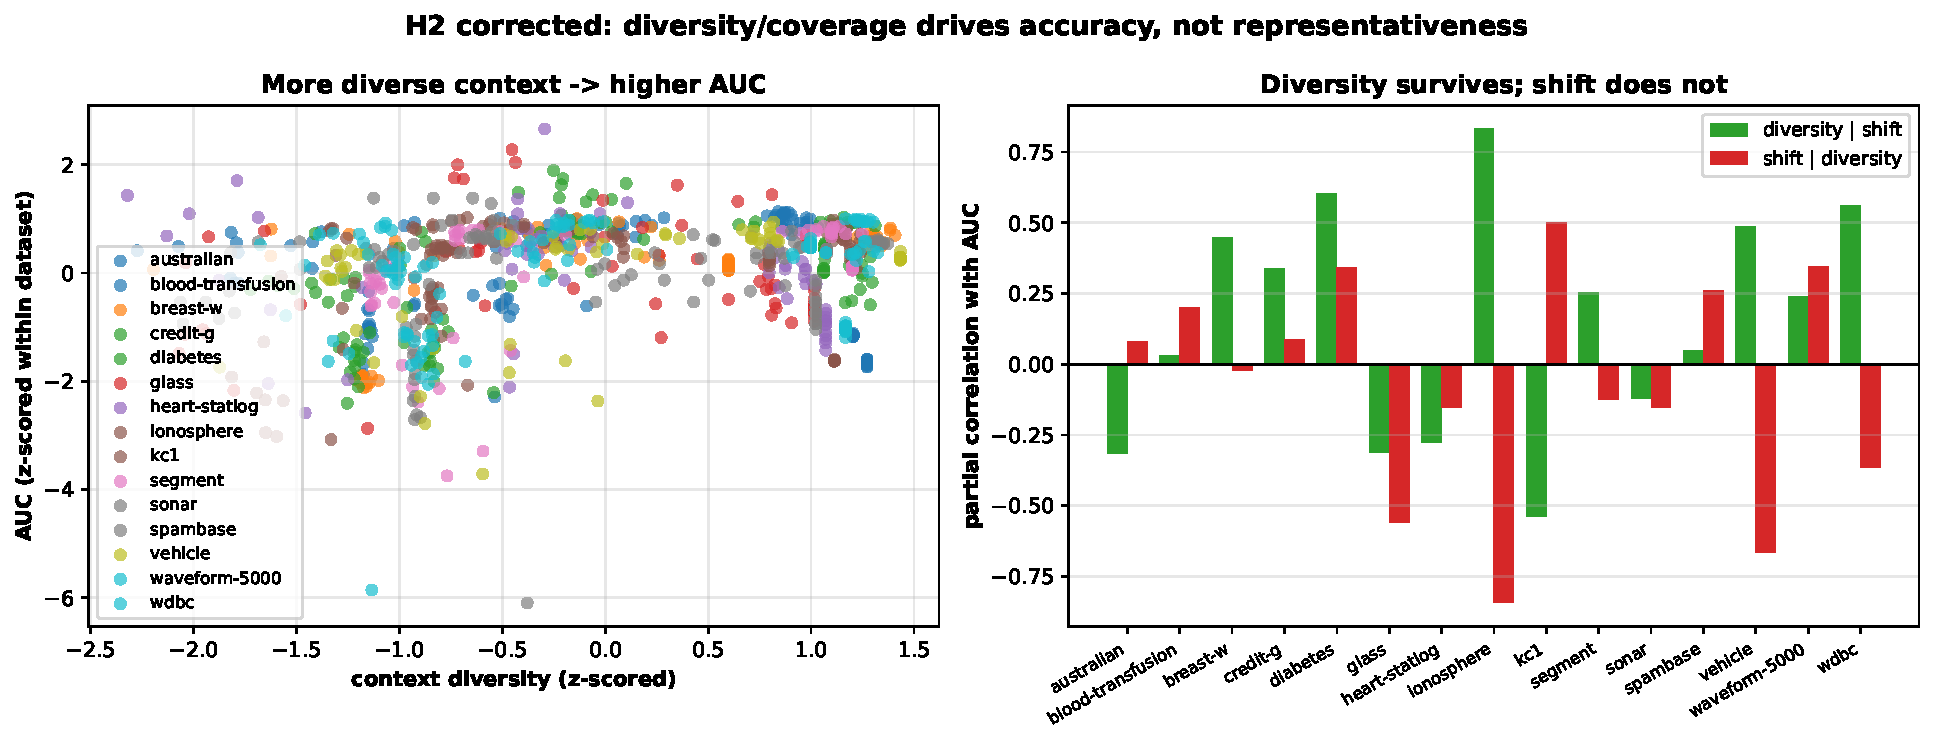
\includegraphics[width=\textwidth]{figures/p2_fig4_disentangle.pdf}
\caption{H2 corrected. Left: across all constructed contexts, AUC tends to rise
with context diversity (z-scored within dataset). Right: partial correlations per
dataset---diversity controlling for shift (green) is positive on most datasets,
while shift controlling for diversity (red) is near zero or negative. In
aggregate (pooled and mixed-effects) diversity is the factor that survives.}
\label{fig:disentangle}
\end{figure}

\section{H3: Selection Cost}

At a fixed budget of $k{=}128$ we compared uniform random selection against
K-Means (nearest training point to each centroid) and farthest-point sampling
(FPS), three seeds each. Table~\ref{tab:selection} reports mean AUC and the mean
time to \emph{choose} the prototypes (separate from inference).

\begin{table}[h]
\centering
\caption{Selection methods at $k{=}128$ (mean ROC AUC $\pm$ 95\% CI over three
seeds).}
\label{tab:selection}
\begin{tabular}{lrrr}
\toprule
Dataset & random AUC & K-Means AUC & FPS AUC \\
\midrule
diabetes           & $.869{\pm}.016$ & $.883{\pm}.007$ & $.877{\pm}.004$ \\
credit-g           & $.745{\pm}.057$ & $.755{\pm}.068$ & $.712{\pm}.024$ \\
vehicle            & $.947{\pm}.004$ & $.944{\pm}.014$ & $.947{\pm}.004$ \\
wdbc               & $.994{\pm}.003$ & $.987{\pm}.004$ & $.994{\pm}.001$ \\
breast-w           & $.994{\pm}.004$ & $.995{\pm}.001$ & $.992{\pm}.002$ \\
blood-transfusion  & $.686{\pm}.008$ & $.720{\pm}.009$ & $.725{\pm}.007$ \\
ionosphere         & $.978{\pm}.004$ & $.974{\pm}.007$ & $.960{\pm}.003$ \\
sonar              & $.893{\pm}.004$ & $.895{\pm}.007$ & $.896{\pm}.004$ \\
glass              & $.952{\pm}.005$ & $.938{\pm}.016$ & $.929{\pm}.016$ \\
australian         & $.924{\pm}.012$ & $.934{\pm}.005$ & $.929{\pm}.008$ \\
heart-statlog      & $.855{\pm}.020$ & $.863{\pm}.005$ & $.868{\pm}.007$ \\
segment            & $.995{\pm}.002$ & $.995{\pm}.001$ & $.997{\pm}.001$ \\
waveform-5000      & $.968{\pm}.001$ & $.958{\pm}.006$ & $.968{\pm}.005$ \\
spambase           & $.971{\pm}.005$ & $.975{\pm}.007$ & $.966{\pm}.001$ \\
kc1                & $.800{\pm}.012$ & $.790{\pm}.019$ & $.771{\pm}.018$ \\
\midrule
\multicolumn{4}{l}{\textit{selection time (mean over datasets):}} \\
\multicolumn{4}{l}{random $\approx 0.0003$\,s \quad FPS $\approx 0.04$\,s
\quad K-Means $\approx 0.22$\,s} \\
\bottomrule
\end{tabular}
\end{table}

\begin{figure}[h]
\centering
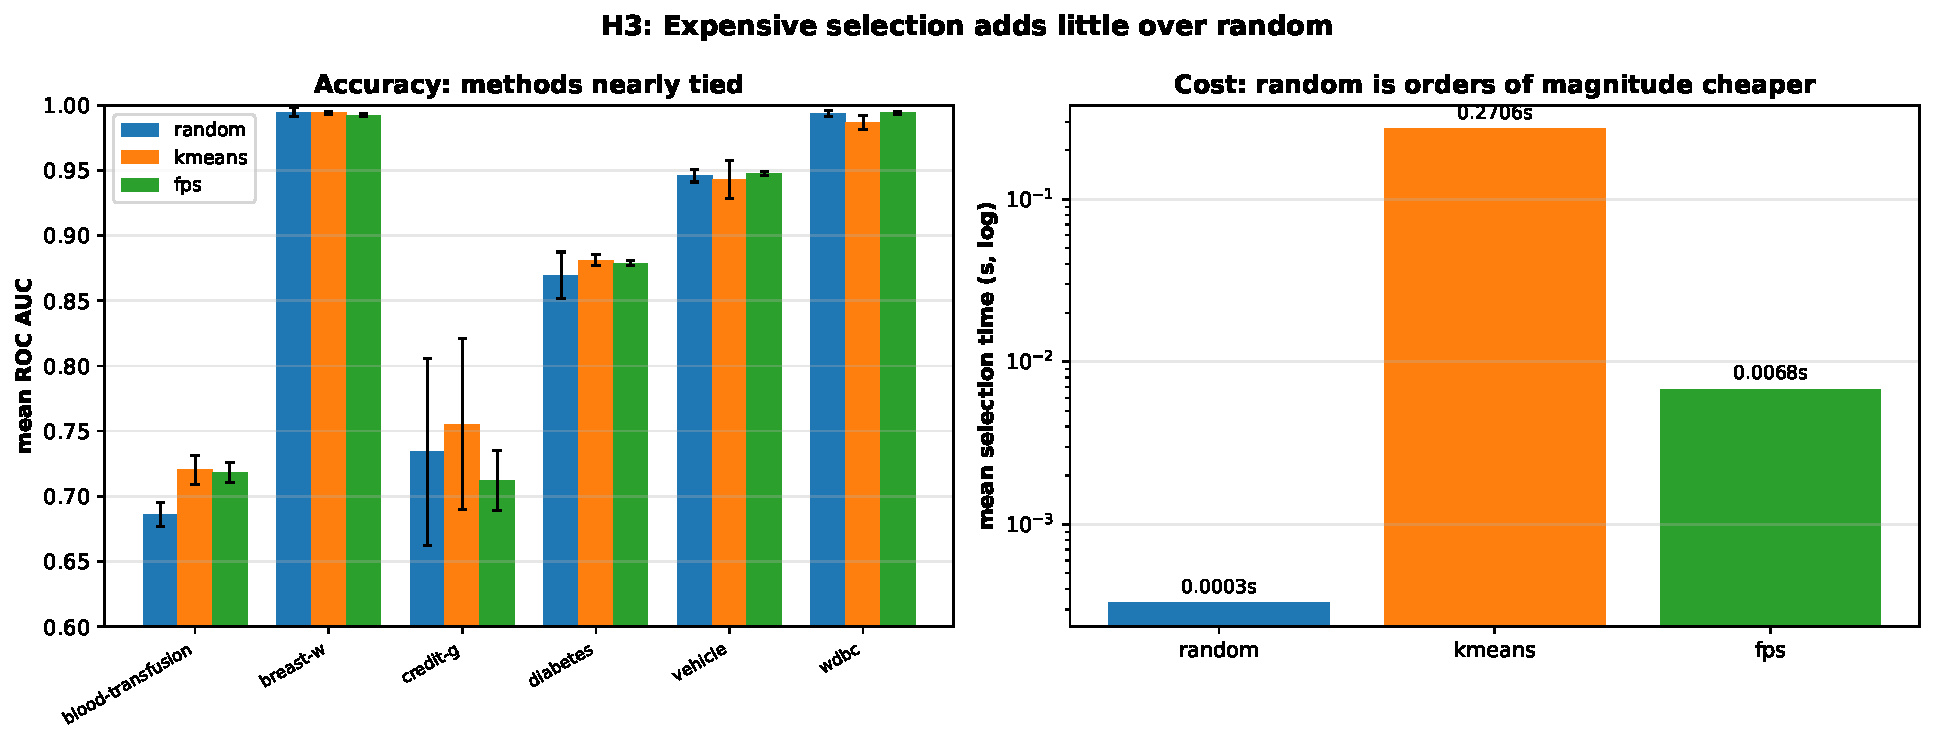
\includegraphics[width=\textwidth]{figures/p2_fig3_selection.pdf}
\caption{Selection methods at $k{=}128$. Accuracy is nearly tied across methods
(left); selection cost differs by two to three orders of magnitude (right).}
\label{fig:selection}
\end{figure}

\textbf{What we observe.} Across all 15 datasets, accuracy differences between the
three methods are small---within about one to three AUC points, and not in a
consistent direction (K-Means marginally ahead on some, FPS or random on others).
The 95\% confidence intervals overlap across methods on most datasets; on
credit-g, where K-Means led random by about one point, the intervals
($0.755{\pm}.068$ vs.\ $0.745{\pm}.057$) overlap heavily, so that gap is not
distinguishable from seed noise. Meanwhile the compute cost differs sharply:
random selection took on the order of $0.0003$\,s versus $\sim$0.22\,s for
K-Means---roughly three orders of magnitude. Given near-equal accuracy, the extra
machinery of K-Means or FPS bought little over drawing rows at random.

This ties back to H2. K-Means and FPS already maximize context diversity---by
spreading prototypes across clusters or across the feature space---which is
exactly the factor H2 identifies as driving accuracy. They perform similarly to
random not despite ignoring distribution matching, but because random already
supplies comparable coverage in expectation. The methods differ mainly in cost,
not in the property that matters.

\section{Supporting: Redundancy and Robustness}

Starting from a random context of $k{=}128$, we either duplicated a fraction of
its rows (adding no new information) or dropped a fraction of them.

\textbf{Redundancy.} Duplicating rows had little effect on most of the 15
datasets: on 13 of them AUC stayed within about 1.5 points up to 70\%
duplication. The clear exception was blood-transfusion, where duplication
steadily hurt ($0.686\rightarrow0.583$), with kc1 and glass showing milder
declines ($\approx-0.015$). So duplicate context rows are mostly harmless when
the signal is strong, but on weak-signal datasets they skew the context and
degrade predictions.

\textbf{Robustness.} Dropping rows degraded accuracy gradually rather than
sharply. Removing 50\% of a 128-row context cost under 1 AUC point on the
stronger datasets (breast-w, diabetes, segment, wdbc) and more on the small or
weak ones (sonar $-0.076$, glass $-0.045$, blood-transfusion $-0.071$). This is
consistent with H1: with fewer rows the context covers less of the space and
predictions get both worse and noisier.

\section{Discussion}

The results fit together into one account of context sampling on small data.
H1 shows that a small context makes TabPFN's prediction unstable---the answer
depends on which rows were drawn---and that enlarging the context removes most of
that instability while also raising accuracy. H2 asks why some contexts are
better, and the controlled experiments give a sharper answer than the initial
correlation suggested: what matters is the context's \emph{diversity / coverage}
of the feature space, not how closely it matches the training distribution.
Matching the marginals, when forced in isolation, actually hurts (because it
reduces coverage); diversity is the factor that survives once the two are
separated. H3 then follows naturally: uniform random sampling covers the space
well in expectation, so it already captures the factor that matters, and the
more expensive selection methods---also diverse, but no more so in ways that
help---add little accuracy at much higher cost.

A larger $k$ helps in the same terms: more rows cover more of the space and are
less subject to an unlucky, narrow draw. Taken together, on small tabular
datasets the useful things to control are the \emph{size and diversity} of the
context, not its distributional fidelity and not the sophistication of the
selection algorithm. Uniform random sampling at a sufficiently large $k$ is a
strong and cheap default because it delivers both.

\section{Conclusion}

We investigated what makes an in-context training set good for TabPFN on small
tabular datasets. (1) Larger contexts are both more accurate and substantially
more stable, with the coefficient of variation of AUC falling several-fold as
$k$ grows. (2) Accuracy correlates with how representative a random context is,
but a controlled experiment overturns that reading: constructing contexts to
match the feature means \emph{lowers} accuracy (by up to 0.5 AUC), and once we
disentangle the two factors, context diversity/coverage predicts accuracy
(mixed-effects $\beta=+0.23$, $p=3\times10^{-12}$) while feature-mean shift does
not ($\beta=-0.01$, $p=0.71$).
(3) K-Means and farthest-point selection---diverse but not
distribution-preserving---match random within about one AUC point at two to three
orders of magnitude more cost. The practical recommendation is direct: use a
sufficiently large random context and spend no effort on expensive selection. The
scientific takeaway is that what a small-data context needs appears to be
coverage of the feature space, not fidelity to its distribution---random sampling
succeeds because it provides the former for free.

\section{Limitations}

\begin{itemize}
\item \textbf{Strength of the causal claim.} Our evidence that diversity, not
representativeness, drives accuracy comes from controlled constructions, partial
correlations, and a mixed-effects model---stronger than a raw correlation, but
still an association over a designed set of contexts rather than a randomized
intervention on a single factor. The per-dataset partial correlations are mixed
(positive on nine of fifteen datasets), so the diversity effect is directionally
dominant in aggregate but not universal. Diversity and coverage are measured with
geometric proxies (mean pairwise distance, covariance log-determinant); a
different proxy could shift the details. We say diversity ``appears to be'' the
driver accordingly.
\item \textbf{Scope of data.} Fifteen small tabular datasets (roughly
200--5000 rows); the findings may not extend to much larger, higher-dimensional,
or non-tabular data. The strength of H2 on any single dataset depends on its
having AUC headroom.
\item \textbf{Model.} A single model (TabPFN v3). Whether the same context
behavior holds for other in-context tabular learners is untested.
\item \textbf{Selection algorithms.} We compare three (random, K-Means, FPS); a
method specifically optimized for context quality could behave differently.
\item \textbf{Representativeness metrics.} Two coarse distances (class-TV,
feature-mean shift); richer divergences (e.g.\ MMD, per-feature KL) might explain
more and are future work.
\item \textbf{Compute.} Runs used a single consumer GPU (RTX 4060); the
selection-time comparison reflects that setup and would differ on other hardware.
\end{itemize}

\section*{Reproducibility}

All numbers are read from logged runs: \texttt{exp14\_context\_sampling\_*.json}
(H1, the correlational part of H2, H3, stress tests),
\texttt{exp15\_controlled\_*.json} (the controlled representativeness test), and
\texttt{exp16\_disentangle\_*.json} (the shift-vs-diversity disentangling), all
under \texttt{experiments/results/}. The mixed-effects model is fit by
\texttt{mixed\_effects\_exp16.py}. Datasets are public OpenML tasks; split seed
and per-block seeds are recorded. Runs used an NVIDIA RTX 4060 GPU.

\begin{thebibliography}{9}
\bibitem{hollmann2024tabpfn}
Hollmann, N., Müller, S., Eggensperger, K., \& Hutter, F. (2024).
Accurate predictions on small data with a tabular foundation model.
\textit{Nature}.
\end{thebibliography}

\end{document}
